\chapter{Method Description}

In this section, the origin DOI method, JDOI method and approximation method based on DOI method are introduced. In section \ref{sec: 2.1},, we describe the origin DOI method. In section \ref{sec: 2.2}, we illustrate the approximation method proposed by \cite{kristensen_adding_2011}. In section \ref{sec: 2.3}, we discuss our estimator to price American options based on JDOI method.

\section{The DOI Variance Reduction Method}
\label{sec: 2.1}

Consider a multi-factor model in which a $d$-dimensional vector of state variables $X(t)$ on a filtered probability space$(\Omega,\mathcal F, \mathbb Q)$, which satisfies the following Stochastic Differential Equations(SDEs)

\begin{equation}\label{general model}
    dX(t) = \mu(t, X(t)) dt + \sigma(t, X(t)) dW(t)
\end{equation}

\noindent where $\mu(t,X(t))$ and $\sigma(t, X(t))$ are drift and diffusion functions under the risk-neutral measure $\mathbb Q$, which also satisfies appropriate growth and Lipschiz conditions such that equation(\ref{general model}) admits a unique strong solution and is Markovian; $W(t)$ is a $d$-dimensional standard Brownian Motion and $t \in [0,T]$.

Besides, we also need to consider the stopping time formulation such that we can apply DOI method to path-dependent options, we shall discuss it later in section \ref{sec: 2.3} when pricing American options.

Let $G(t, X(t))$ be the price of derivative written on $X(t)$. Suppose it's sufficiently smooth and current state $X(t) = x$, we define the infinitesimal generator $\mathcal L$ associated with equation(\ref{general model})to be

\begin{equation}
    (\mathcal{L} G)(t, X(t))=\frac{\partial V}{\partial t} + \sum_{i=1}^{d} \mu(t, x) \frac{\partial V}{\partial x}+\frac{1}{2} \sum_{i, j=1}^{d} \sigma_{i j}^2(t,x) \frac{\partial^2 V}{\partial x_i x_j}
\end{equation}
\section{Approximation Method based on DOI method}
\label{sec: 2.2}

\section{JDOI method}
\label{sec: 2.3}
  
\normalsize 

% \begin{figure}[htp]
% \centering
% 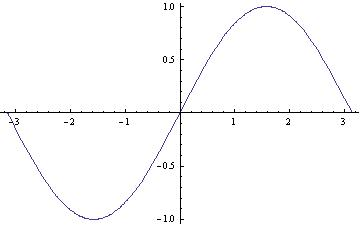
\includegraphics{sin_x.jpg}
% \caption{Transverse momentum distributions}\label{fig:erptsqfit}
% \end{figure}

